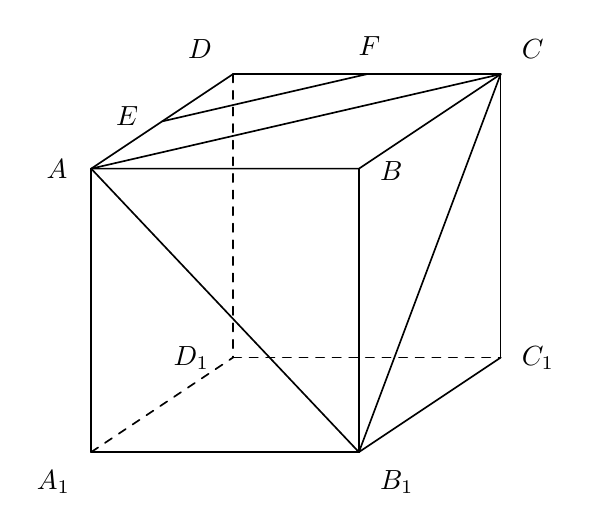
\begin{tikzpicture}[line width=.6pt,line join=round,line cap=round]
\coordinate (A) at (0,3.6);
\coordinate (B) at (3.4,3.6);
\coordinate (C) at (5.2,4.8);
\coordinate (D) at (1.8,4.8);
\coordinate (F) at (3.5,4.8);
\coordinate (E) at (0.9,4.2);
\coordinate (A1) at (0,0);
\coordinate (B1) at (3.4,0);
\coordinate (C1) at (5.2,1.2);
\coordinate (D1) at (1.8,1.2);
% top face
\draw[solid] (D) -- (F) -- (C);
\draw[solid] (A) -- (B) -- (C);
\draw[solid] (A) -- (D);
% verticals
\draw[solid] (A) -- (A1);
\draw[solid] (B) -- (B1);
\draw[solid] (C) -- (C1);
\draw[dashed] (D) -- (D1);
% bottom face
\draw[solid] (A1) -- (B1);
\draw[dashed] (D1) -- (C1);
\draw[dashed] (A1) -- (D1);
\draw (B1)--(C1);
% interior segments
\draw[solid] (A) -- (C);
\draw[solid] (E) -- (F);
\draw[solid] (A) -- (B1);
\draw[solid] (C) -- (B1);
% labels
\node[left,xshift=-5pt] at (A) {$A$};
\node[right,xshift=4pt,yshift=-1pt] at (B) {$B$};
\node[above right,xshift=4pt,yshift=2pt] at (C) {$C$};
\node[above left,xshift=-4pt,yshift=2pt] at (D) {$D$};
\node[left,xshift=-5pt,yshift=2pt] at (E) {$E$};
\node[above,xshift=1pt,yshift=3pt] at (F) {$F$};
\node[below left,xshift=-4pt,yshift=-3pt] at (A1) {$A_{1}$};
\node[below right,xshift=4pt,yshift=-3pt] at (B1) {$B_{1}$};
\node[right,xshift=4pt] at (C1) {$C_{1}$};
\node[left,xshift=-5pt] at (D1) {$D_{1}$};
\end{tikzpicture}
